%----------------------------------------------------------------------------------------
%   LAGRANGIAN POINTS
%----------------------------------------------------------------------------------------

\section{Computation of the Lagrangian points}
\subsection{Introduction}
Given a set of forces which apply to an object in the plane, our goal is to compute the equilibrium positions of this object. We will restrain ourselves to three kind of interactions: elastic, centrifugal and gravitational forces. We will need the previously written Newton-Raphson method, which will be applied to the resultant force. As a result, we will obtain the roots of this three-dimensional function, corresponding to the equilibrium positions.

\subsection{Forces}
Before explaining and analysing the method, we need to express both the general form of the forces and their Jacobian matrices. Each force will be parameterized with an integer - the intensity - and their origin.

We will start with the elastic force, which represent a spring action on an object. In a one dimensional space, this force is expressed by the following formula:
\[\vec{f}_c = -k (l - l_0)\vec{x},\]
with $l$ the spring length and $l_0$ its free length.

In the plane $(O, \vec{x}, \vec{y})$, this force can be reduced using orthogonals projections to the following form:
\[f_e:\begin{pmatrix}x\\y\end{pmatrix}\rightarrow \begin{pmatrix}\frac{-k(x-x_0)}{\sqrt[]{(x-x_0)^2+(y-y_0)^2}}\\\frac{-k(y-y_0)}{\sqrt[]{(x-x_0)^2+(y-y_0)^2}}\end{pmatrix},\]
where $\begin{pmatrix}x_0\\y_0\end{pmatrix}$ is the origin coordinate and $k$ the intensity.

We can now express the $f_e$ Jacobian matrix:
\[H_{f_e}:\begin{pmatrix}x\\y\end{pmatrix}\rightarrow \begin{pmatrix}
\frac{(y_0-y)^2}{((x_0-x)^2+(y_0-y)^2)^\frac{3}{2}} & 
\frac{(x_0-x)(y_0-y)}{((x_0-x)^2+(y_0-y)^2)^\frac{3}{2}}\\
-\frac{(x_0-x)(y_0-y)}{((x_0-x)^2+(y_0-y)^2)^\frac{3}{2}} & 
\frac{(x_0-x)^2}{((x_0-x)^2+(y_0-y)^2)^\frac{3}{2}}
\end{pmatrix}\]

Since the force expressions have already been given in the subject, we will only provide the forms of the Jacobian matrices for the centrifugal and gravitational forces:
\[H_{f_c}:\begin{pmatrix}x\\y\end{pmatrix}\rightarrow \begin{pmatrix}
k & 0\\
0 & k
\end{pmatrix}\]

\[H_{f_g}:\begin{pmatrix}x\\y\end{pmatrix}\rightarrow \begin{pmatrix}
\frac{k(2x_0^2 - y_0^2 - 4x_0x + 2x^2 + 2y_0y - y^2)}{((x_0 - x)^2 + (y_0 - y)^2)^\frac{5}{2}} &
\frac{3k(x_0 - x)(y_0 - y)}{((x_0 - x)^2 + (y_0 - y)^2)^\frac{5}{2}}\\
\frac{3k(x_0 - x)(y_0 - y)}{((x_0 - x)^2 + (y_0 - y)^2)^\frac{5}{2}} &
-\frac{c (x_0^2 - 2 y_0^2 - 2 x_0 x + x^2 + 4 y_0 y - 2 y^2)}{((x_0 - x)^2 + (y_0 - y)^2)^\frac{5}{2}}
\end{pmatrix}\]

\paragraph{Implementation} The implementation use a functionnal programming approach, which means that we use a kind of functions which will build and return a function as expression. This allow us to be more versatile by storing and using the function itself rather than using a general function, and to give it as a parameter to the Newton-Raphson method for example.

\paragraph{Tests} The tests check in particular cases the validity of the result for one force. In particular, we check for the gravitational force that the norm is invariant by rotation around the origin. Moreover, these tests rose the issue of dividing by a norm equal to zero. We handle this case by setting the value to the asymptotic value of the function in this point (either infinite or a constant). % Bring examples...

\subsection{Results}
\subsubsection{First approach}
We consider the following case:
\begin{itemize}
  \item Two gravitational forces with coefficients $1$ (resp. $0.01$) and originating from $\begin{pmatrix}0\\0\end{pmatrix}$ (resp. $\begin{pmatrix}1\\0\end{pmatrix}$).
  \item A centrifugal force with coefficient $1$ at the barycenter of the two masses, i.e., at $\begin{pmatrix}\frac{0.01}{1.01}\\0\end{pmatrix}$.
\end{itemize}

We can easily plot the situation using the norm of the resultant force. So we get the Figure~\vref{fig:resultant_force_norm}. From above, the graph is more explicit, as shown in the Figure~\vref{fig:equilibrium}. The situation is similar to the Earth rotation around the Sun. Centrifugal force and gravitational attraction by the Sun are applied to the Earth. The centrifugal force applied to the barycenter of the two bodies is characteristic of a two-body interaction.

\begin{figure}[ht]
\centering 
\subfloat[3D shape]{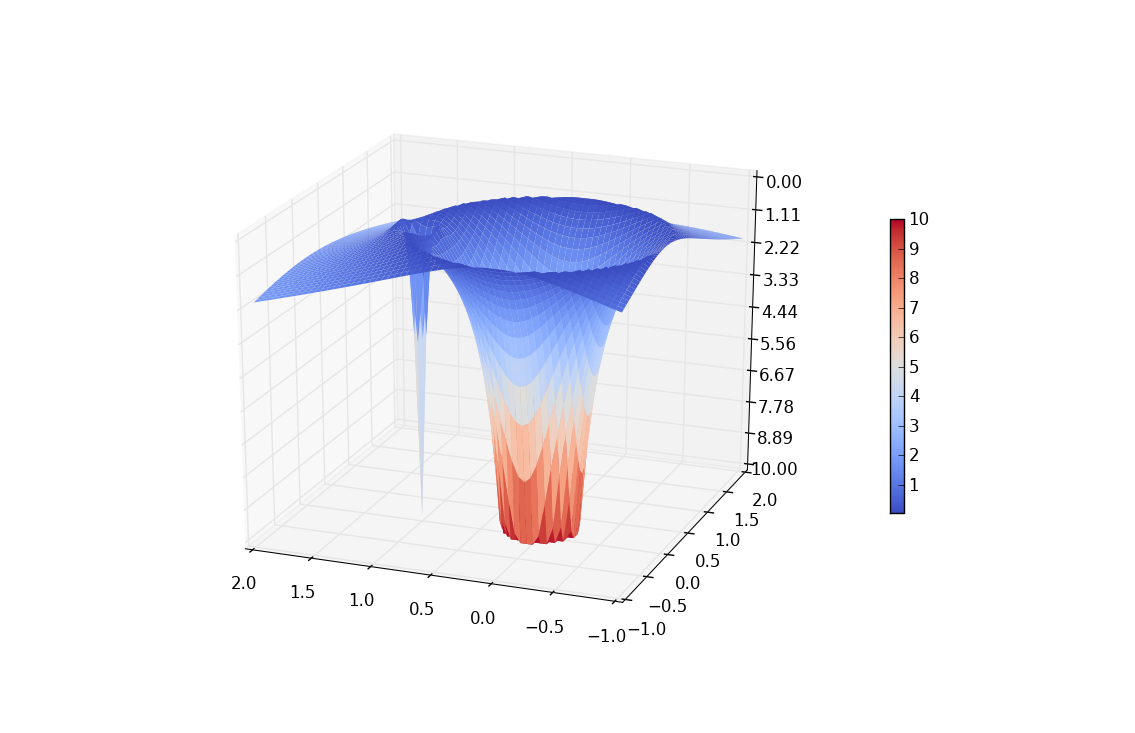
\includegraphics[width=.6\columnwidth]{resultant_force_norm}\label{fig:resultant_force_norm}}
\subfloat[Equilibrium]{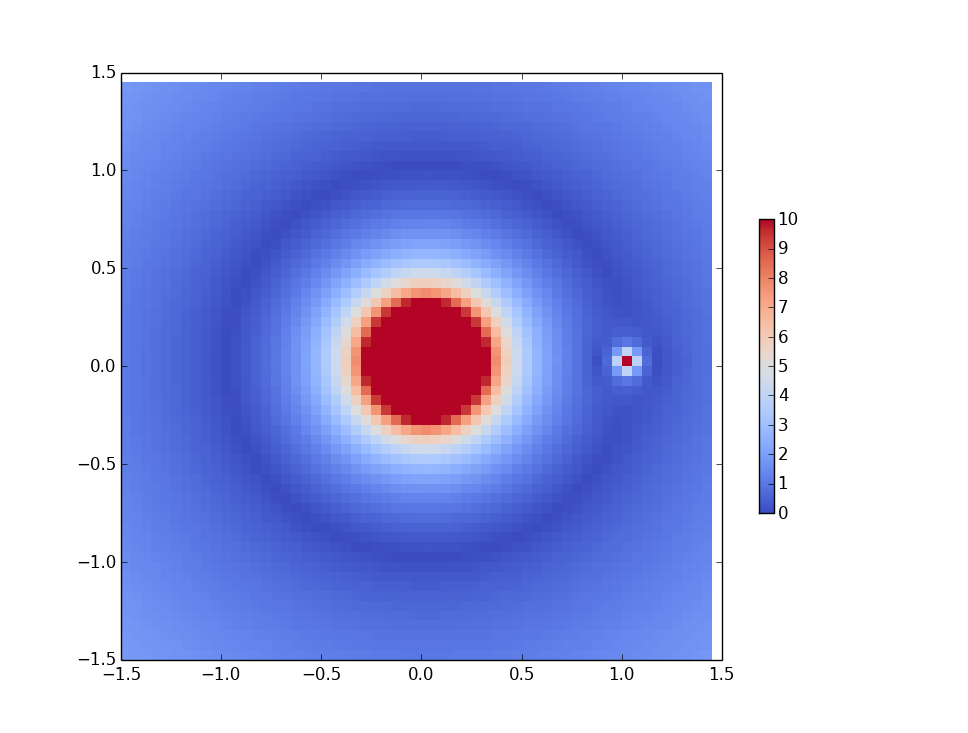
\includegraphics[width=.45\columnwidth]{equilibrium}\label{fig:equilibrium}}
\caption[Resultant force norm]{Resultant force norm}
\end{figure}

\subsubsection{Lagrangian points}
The main issue is that the Newton-Raphson method can only compute one root while we seem to have an infinite number of roots. We can call the algorithm by specifying a step over the whole grid. We will see that in this kind of interaction, the equilibrium points are particular and well-known as the Lagrangian points.

It is not obvious with the last example that only five points correspond to an equilibrium situation. However, we can modify a bit the datas to make this phenomenon more clear and spread the values with the logarithm, as in Figure~\vref{fig:lagrange_points}.

\begin{figure}[ht]
  \centering
  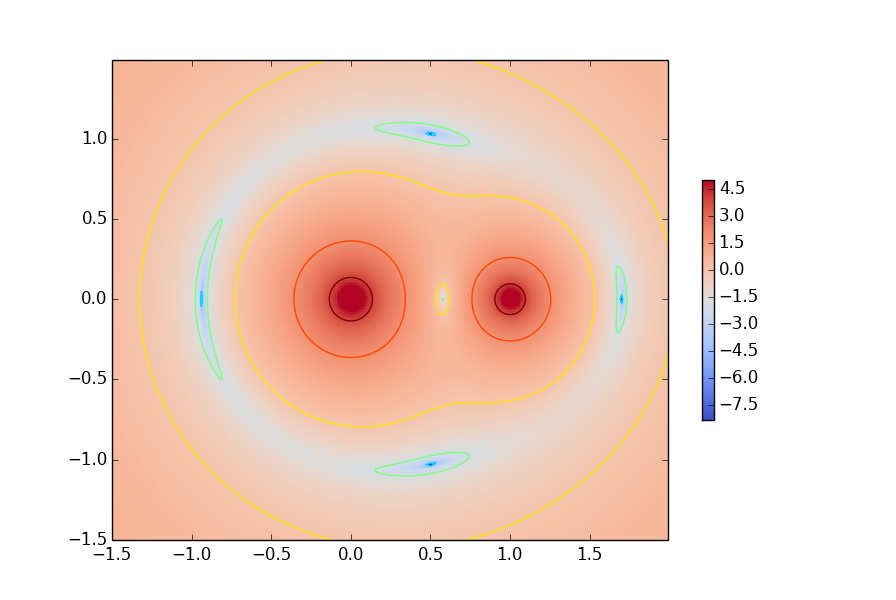
\includegraphics[width=0.8\columnwidth]{lagrange_points} 
  \caption[Lagrange points]{Lagrangian points.}
  \label{fig:lagrange_points}
\end{figure}

As the Newton-Raphson algorithm follows the slope of the curve, we can call it on equireparted points on the grid, distant by a fixed step we will note $\tau$. The algorithm must work in a closed domain. Moreover, at each iteration, the algorithm will output a position corresponding to a root. Assuming that we will perform enough iterations to find at least all the roots, we must be able to determine a maximal precision on a root coordinate. The minimal distance between two distinct roots, noted $\varepsilon$, will be another parameter of this algorithm.